\section{实验三：\texttt{TCP} 连接重置}

\subsection{实验环境与网络配置}

本实验在 WSL2 中使用 Docker Compose 搭建隔离网络。拓扑包含攻击者、用户、路由器、受害者服务器和正常服务器。攻击者、用户分别位于不同网段；两台服务器位于同一服务器网段，由路由器转发用户与服务器之间的流量。各节点地址如表~\ref{tab:task3-network} 所示。

\begin{table}[H]
    \centering
    \caption{\texttt{TCP} 连接重置实验的实际网络配置}
    \label{tab:task3-network}
    \renewcommand{\arraystretch}{1.2}
    \begin{tabularx}{\linewidth}{l l l X}
        \toprule
        节点 & 网段侧 & IPv4 地址 & 默认路由 \\
        \midrule
        Attacker & 攻击者网段 & \texttt{192.168.2.100/24} & \texttt{192.168.2.10} \\
        User & 用户网段 & \texttt{192.168.3.100/24} & \texttt{192.168.3.10} \\
        Router & 攻击者侧 & \texttt{192.168.2.10/24} & -- \\
        Router & 用户侧 & \texttt{192.168.3.10/24} & -- \\
        Router & 服务器侧 & \texttt{192.168.4.10/24} & -- \\
        Victim Server & 服务器网段 & \texttt{192.168.4.105/24} & \texttt{192.168.4.10} \\
        Normal Server & 服务器网段 & \texttt{192.168.4.106/24} & \texttt{192.168.4.10} \\
        \bottomrule
    \end{tabularx}
\end{table}

路由器开启 IPv4 转发，并使用 Linux 流量控制（\texttt{tc}）把用户侧和服务器侧入口的 IPv4 报文镜像到攻击者侧。Docker 网络关闭源地址伪装，因而镜像报文仍保留 User 和服务器的原始 IP 地址。Attacker 上的 Scapy 脚本只处理从受害者服务器发往 User 的 \texttt{TCP} 报文，并从中读取端口和确认号。

\subsection{攻击前的连通性检查}

开始攻击前，User 分别访问受害者服务器和正常服务器。\texttt{HTTP} 请求均得到 \texttt{HTTP/1.1 200 OK}，\texttt{SSH}、\texttt{Telnet} 和 \texttt{FTP} 也均可建立连接并完成登录，作为后续对照。以下截图中的标记标出了相关客户端命令。\texttt{HTTP} 检查结果如图~\ref{fig:task3-http-before} 所示。

\begin{figure}[H]
    \centering
    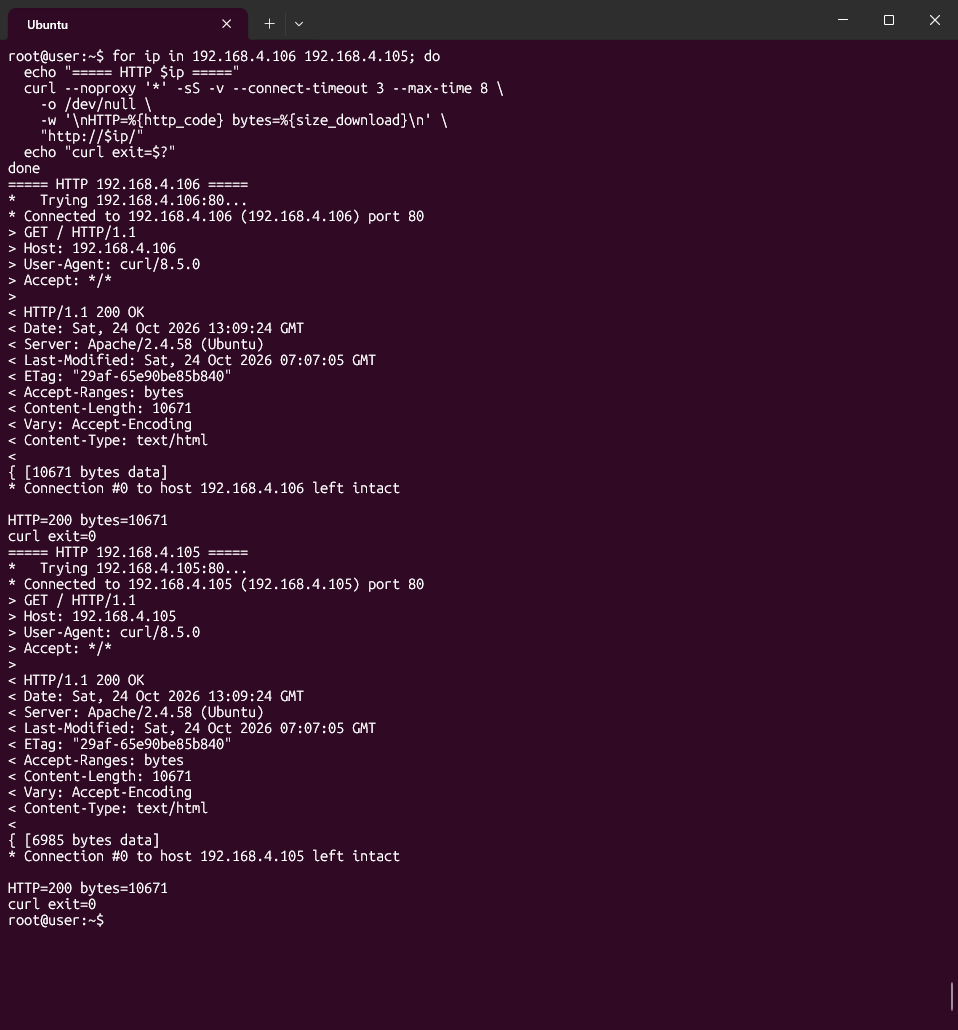
\includegraphics[width=0.86\linewidth]{figures/task3/http_before_attack.png}
    \caption{攻击前，User 能正常访问两台服务器的 \texttt{HTTP} 服务}
    \label{fig:task3-http-before}
\end{figure}

\texttt{Telnet} 登录结果如图~\ref{fig:task3-telnet-before} 所示，User 先后登录了正常服务器和受害者服务器，并能在两端执行命令。

\begin{figure}[H]
    \centering
    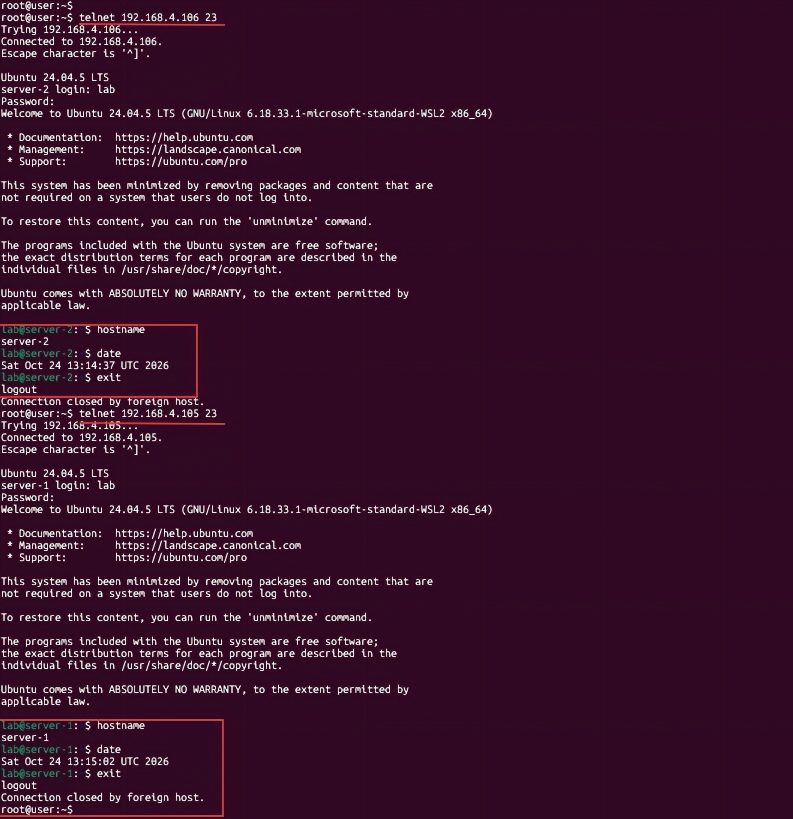
\includegraphics[width=0.78\linewidth]{figures/task3/telnet_before_attack(1).png}
    \caption{攻击前，User 分别成功登录两台服务器的 \texttt{Telnet} 服务}
    \label{fig:task3-telnet-before}
\end{figure}

\texttt{SSH} 检查中，User 分别连接到两台服务器并显示各自的主机名，说明攻击前两条 \texttt{SSH} 连接均可正常使用，如图~\ref{fig:task3-ssh-before} 所示。

\begin{figure}[H]
    \centering
    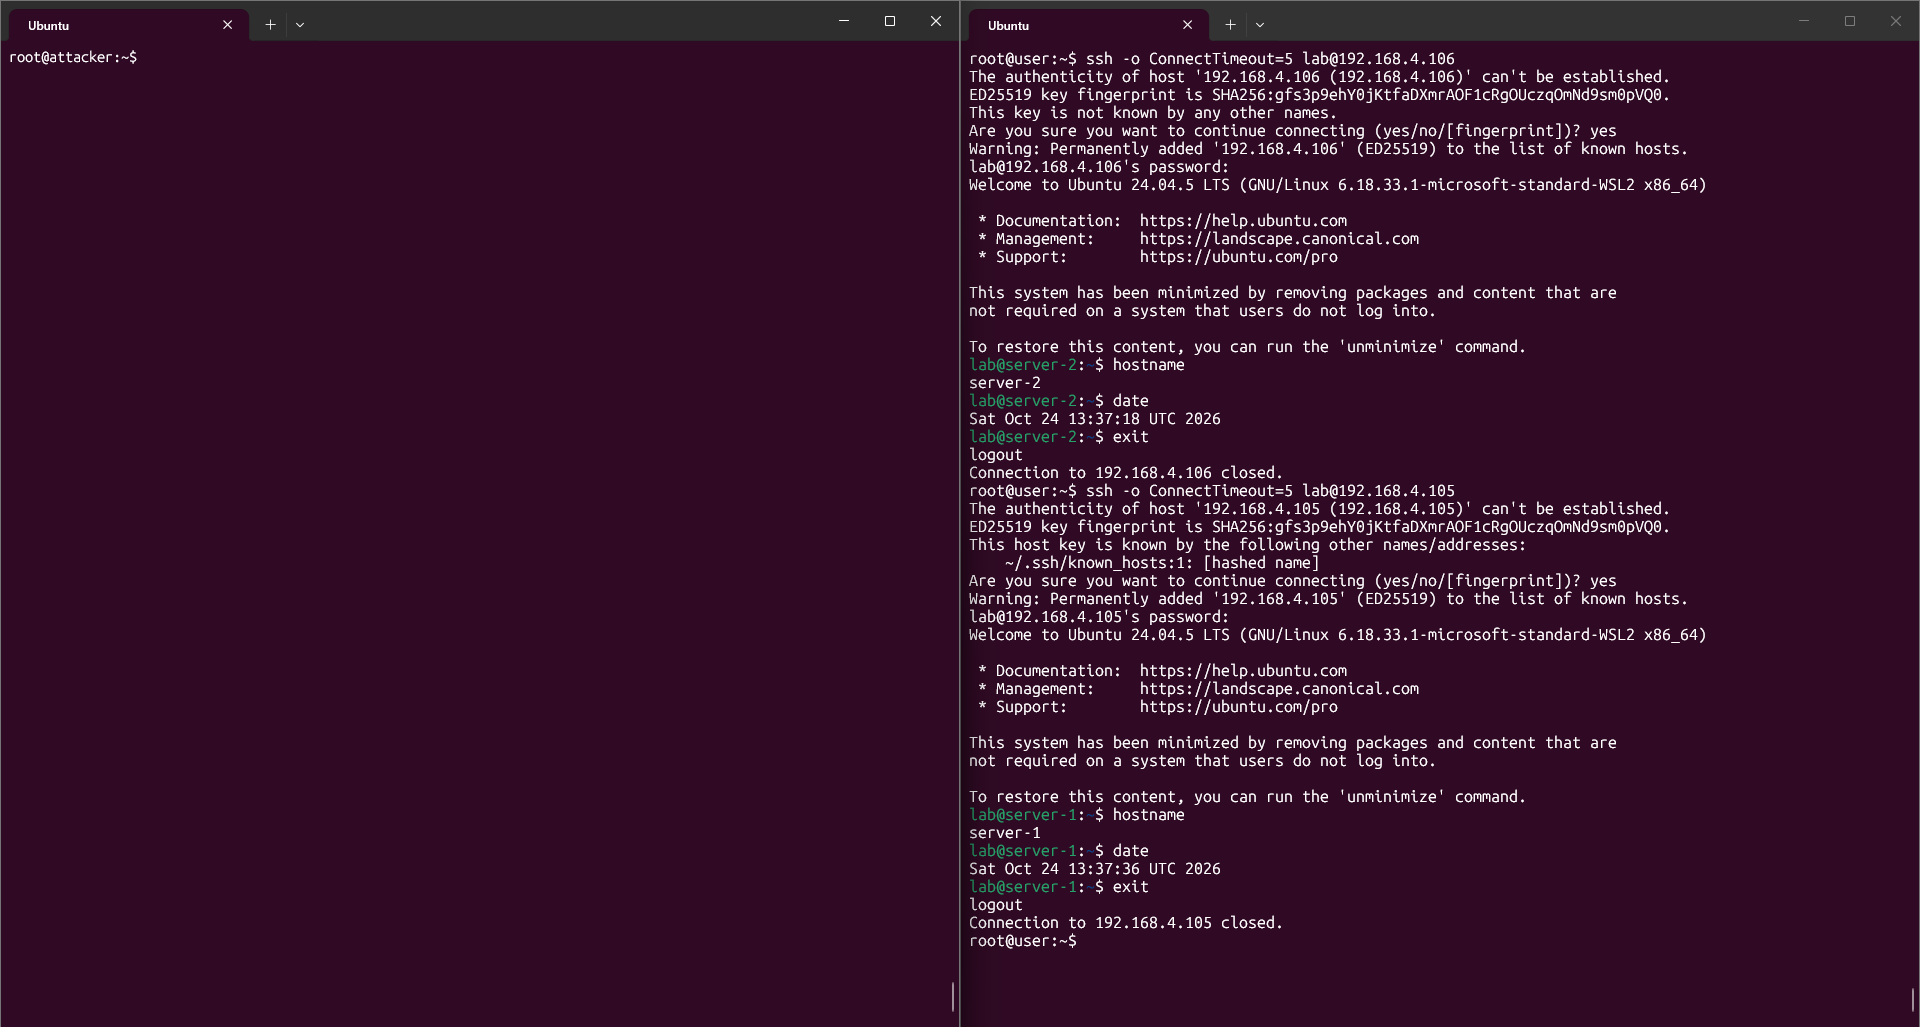
\includegraphics[trim=720bp 0 0 0,clip,width=0.88\linewidth]{figures/task3/ssh_before_attack.png}
    \caption{攻击前，User 分别通过 \texttt{SSH} 登录正常服务器和受害者服务器}
    \label{fig:task3-ssh-before}
\end{figure}

\texttt{FTP} 检查中，两台服务器均返回登录成功和目录列表，结果如图~\ref{fig:task3-ftp-before} 所示。

\begin{figure}[H]
    \centering
    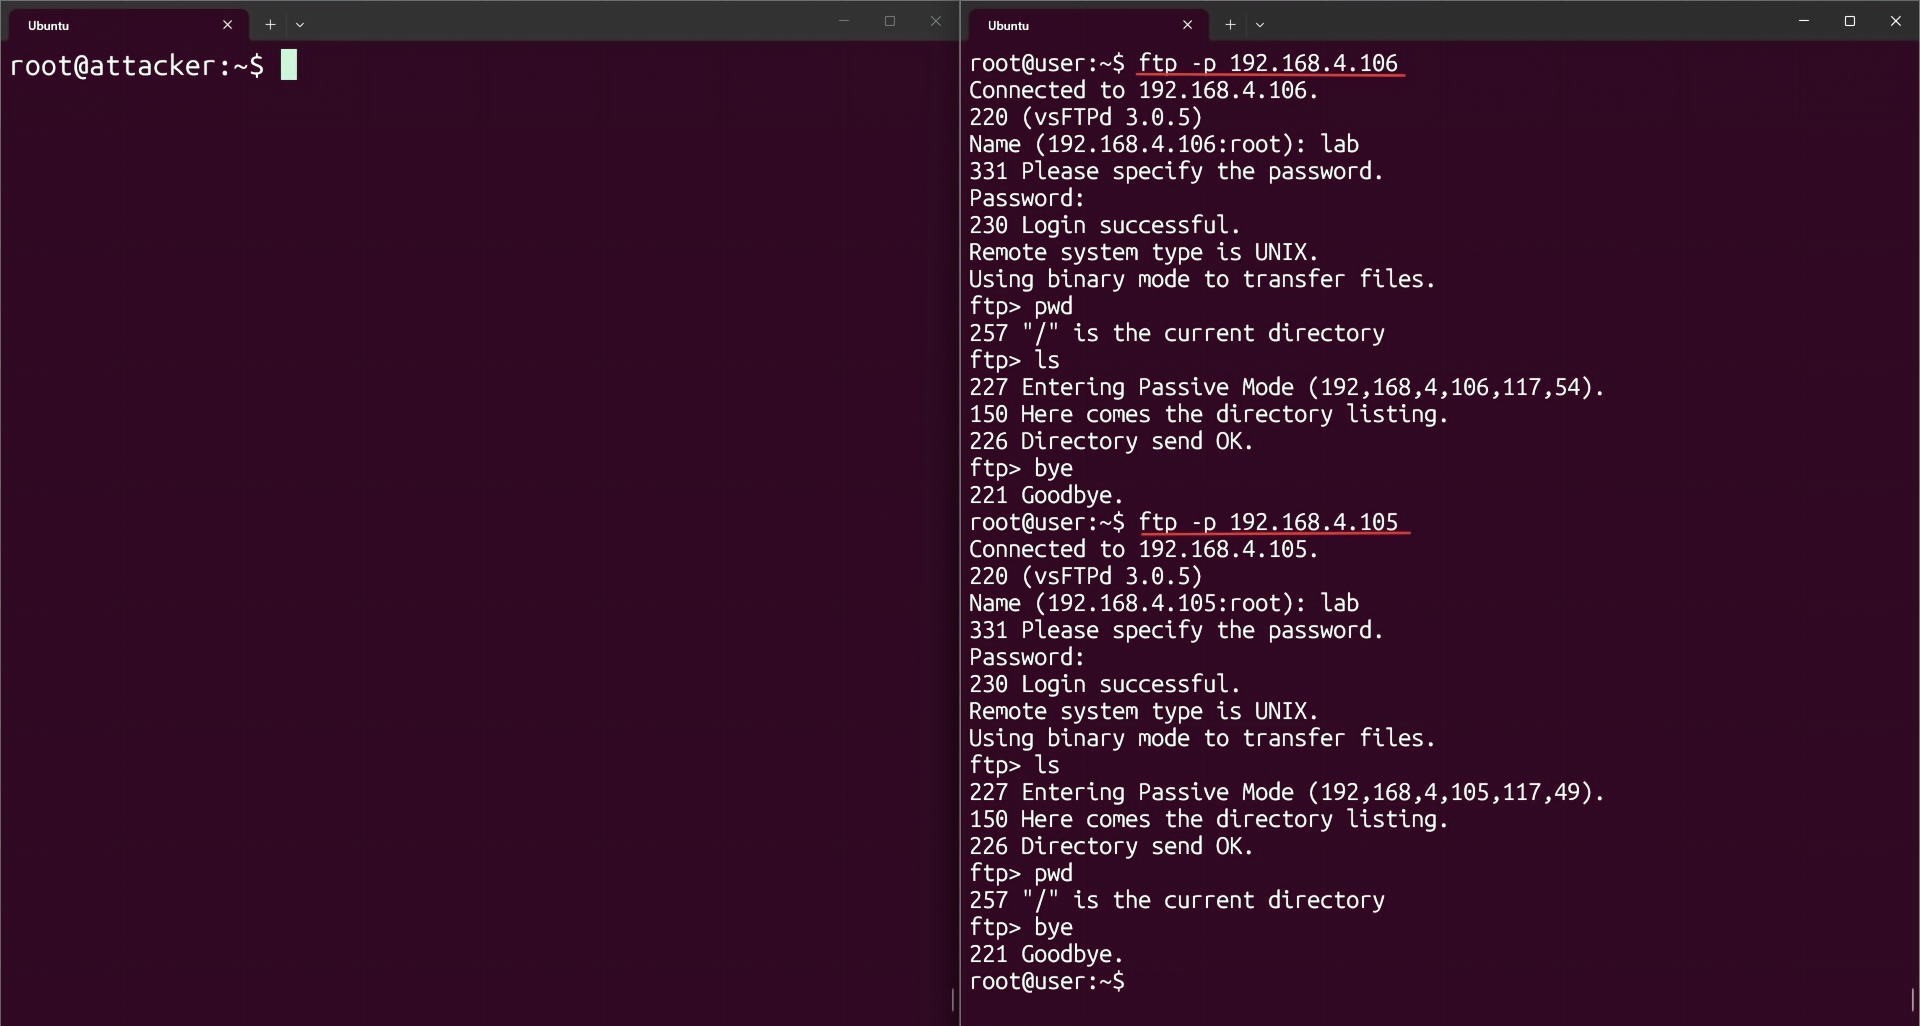
\includegraphics[trim=720bp 0 0 0,clip,width=0.88\linewidth]{figures/task3/ftp_before_attack(1).png}
    \caption{攻击前，User 均可登录两台服务器的 \texttt{FTP} 服务}
    \label{fig:task3-ftp-before}
\end{figure}

\subsection{监听流量并构造 \texttt{TCP} RST 报文}

在 Attacker 上运行 Scapy 监听脚本后，脚本使用如下过滤条件捕获从受害者服务器发往 User 的 \texttt{TCP} 报文：

\begin{lstlisting}[language=Python,caption={捕获服务器发往 User 的 \texttt{TCP} 流量}]
capture_filter = (
    "tcp and src host 192.168.4.105 "
    "and dst host 192.168.3.100"
)
\end{lstlisting}

回调函数从捕获报文中读取 \texttt{TCP} 源、目的端口和确认号，将 IP 地址及端口方向反转，并把服务器报文中的确认号作为伪造 RST 的序列号。脚本只对带 ACK 标志的报文发送 RST，核心处理如下：

\begin{lstlisting}[language=Python,caption={根据捕获到的确认号构造 \texttt{TCP} RST 报文}]
def packet_callback(packet):
    if not (packet.haslayer(IP) and packet.haslayer(TCP)):
        return

    tcp_layer = packet[TCP]
    if not (int(tcp_layer.flags) & 0x10):
        return

    reset_packet = (
        IP(src=USER_IP, dst=VICTIM_IP)
        / TCP(
            sport=int(tcp_layer.dport),
            dport=int(tcp_layer.sport),
            flags="R",
            seq=int(tcp_layer.ack),
        )
    )
    send(reset_packet, iface=ATTACKER_INTERFACE, verbose=False)

sniff(
    iface=ATTACKER_INTERFACE,
    filter=CAPTURE_FILTER,
    prn=packet_callback,
    store=False,
)
\end{lstlisting}

脚本启动后，User 分别使用 \texttt{HTTP}、\texttt{SSH}、\texttt{Telnet} 和 \texttt{FTP} 访问正常服务器及受害者服务器。攻击者终端显示其持续捕获服务器响应并发送以 User 为源地址、受害者服务器为目的地址的 RST 报文。

\subsection{不同 \texttt{TCP} 服务的攻击结果}

\subsubsection{\texttt{Telnet}、\texttt{SSH} 与 \texttt{FTP}}

\texttt{Telnet} 对照结果显示，攻击期间 User 仍能登录正常服务器 \texttt{192.168.4.106}；连接受害者服务器 \texttt{192.168.4.105} 时，服务器登录过程被中断，连接随即关闭，如图~\ref{fig:task3-telnet-after} 所示。

\begin{figure}[H]
    \centering
    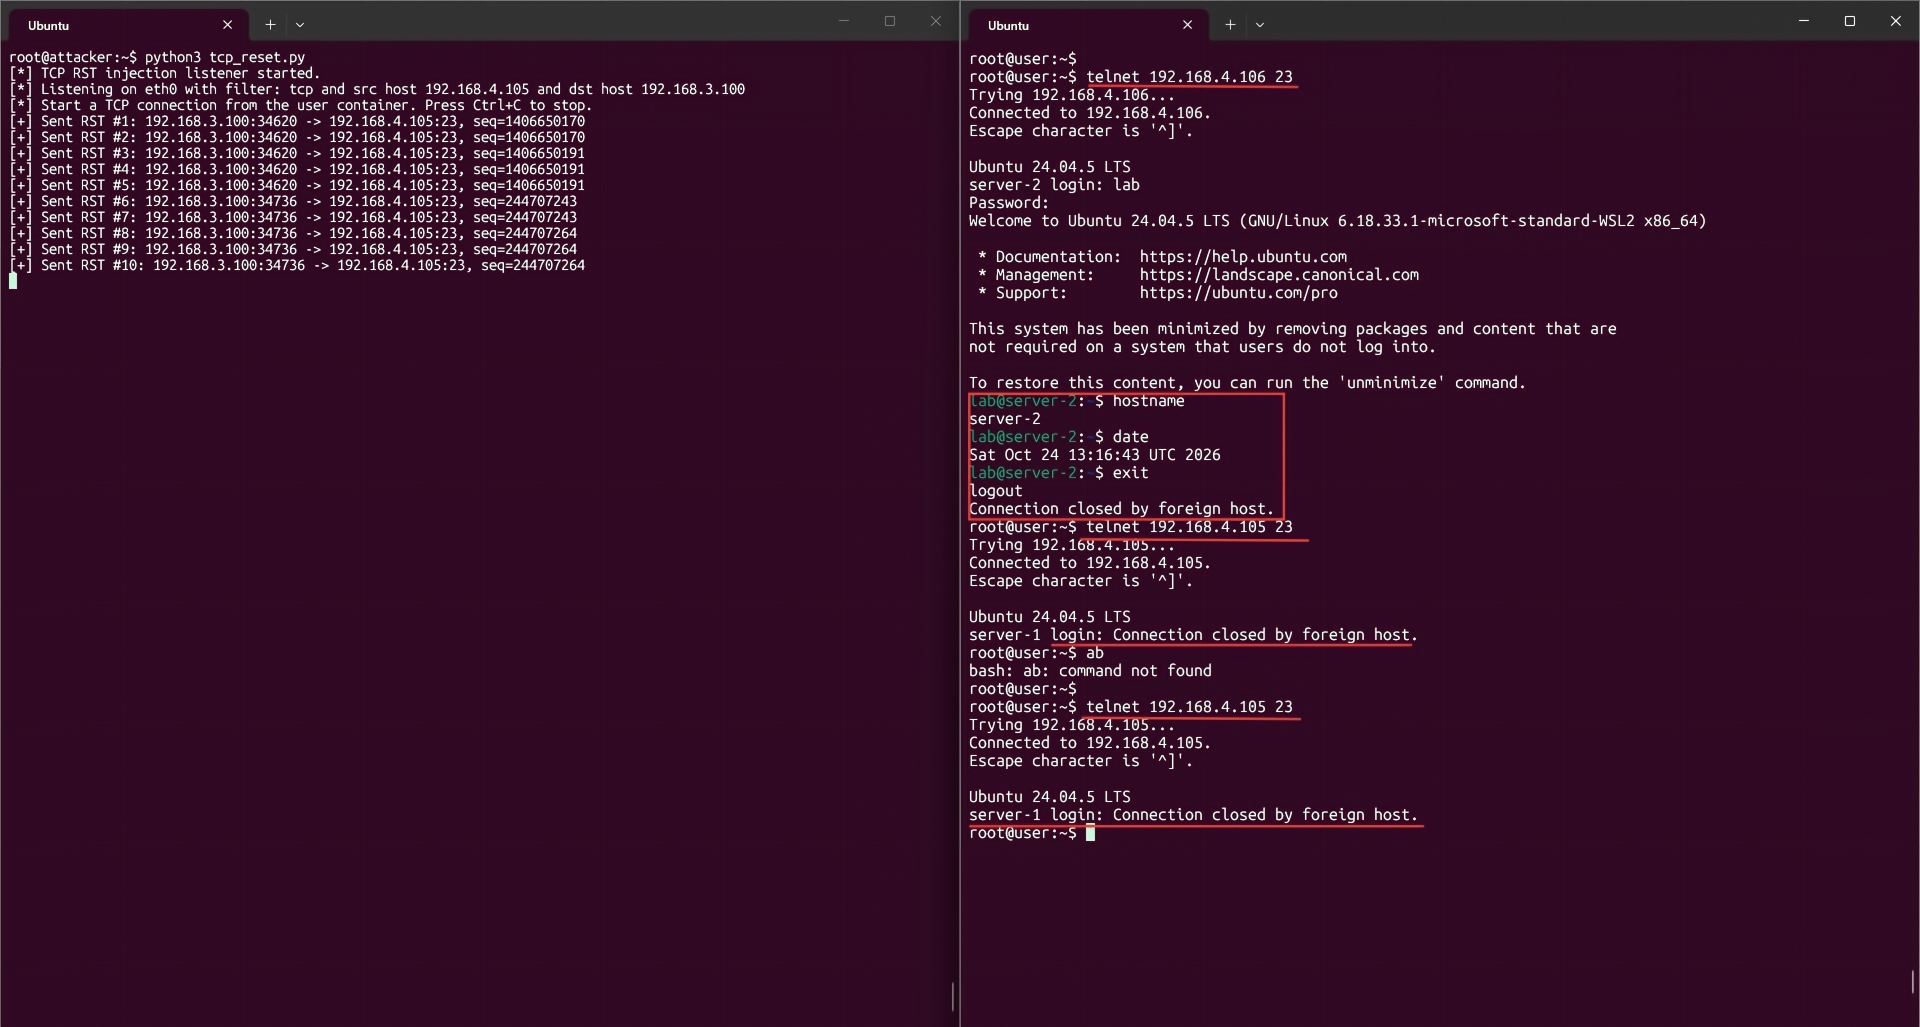
\includegraphics[trim=720bp 0 0 0,clip,width=0.88\linewidth]{figures/task3/telnet_after_attack(1).png}
    \caption{\texttt{TCP} 重置期间，正常服务器 \texttt{Telnet} 可用，受害者服务器连接被重置}
    \label{fig:task3-telnet-after}
\end{figure}

\texttt{SSH} 的结果与 \texttt{Telnet} 一致：正常服务器仍可登录，而连接受害者服务器时出现 \texttt{Connection reset by 192.168.4.105}，如图~\ref{fig:task3-ssh-after} 所示。

\begin{figure}[H]
    \centering
    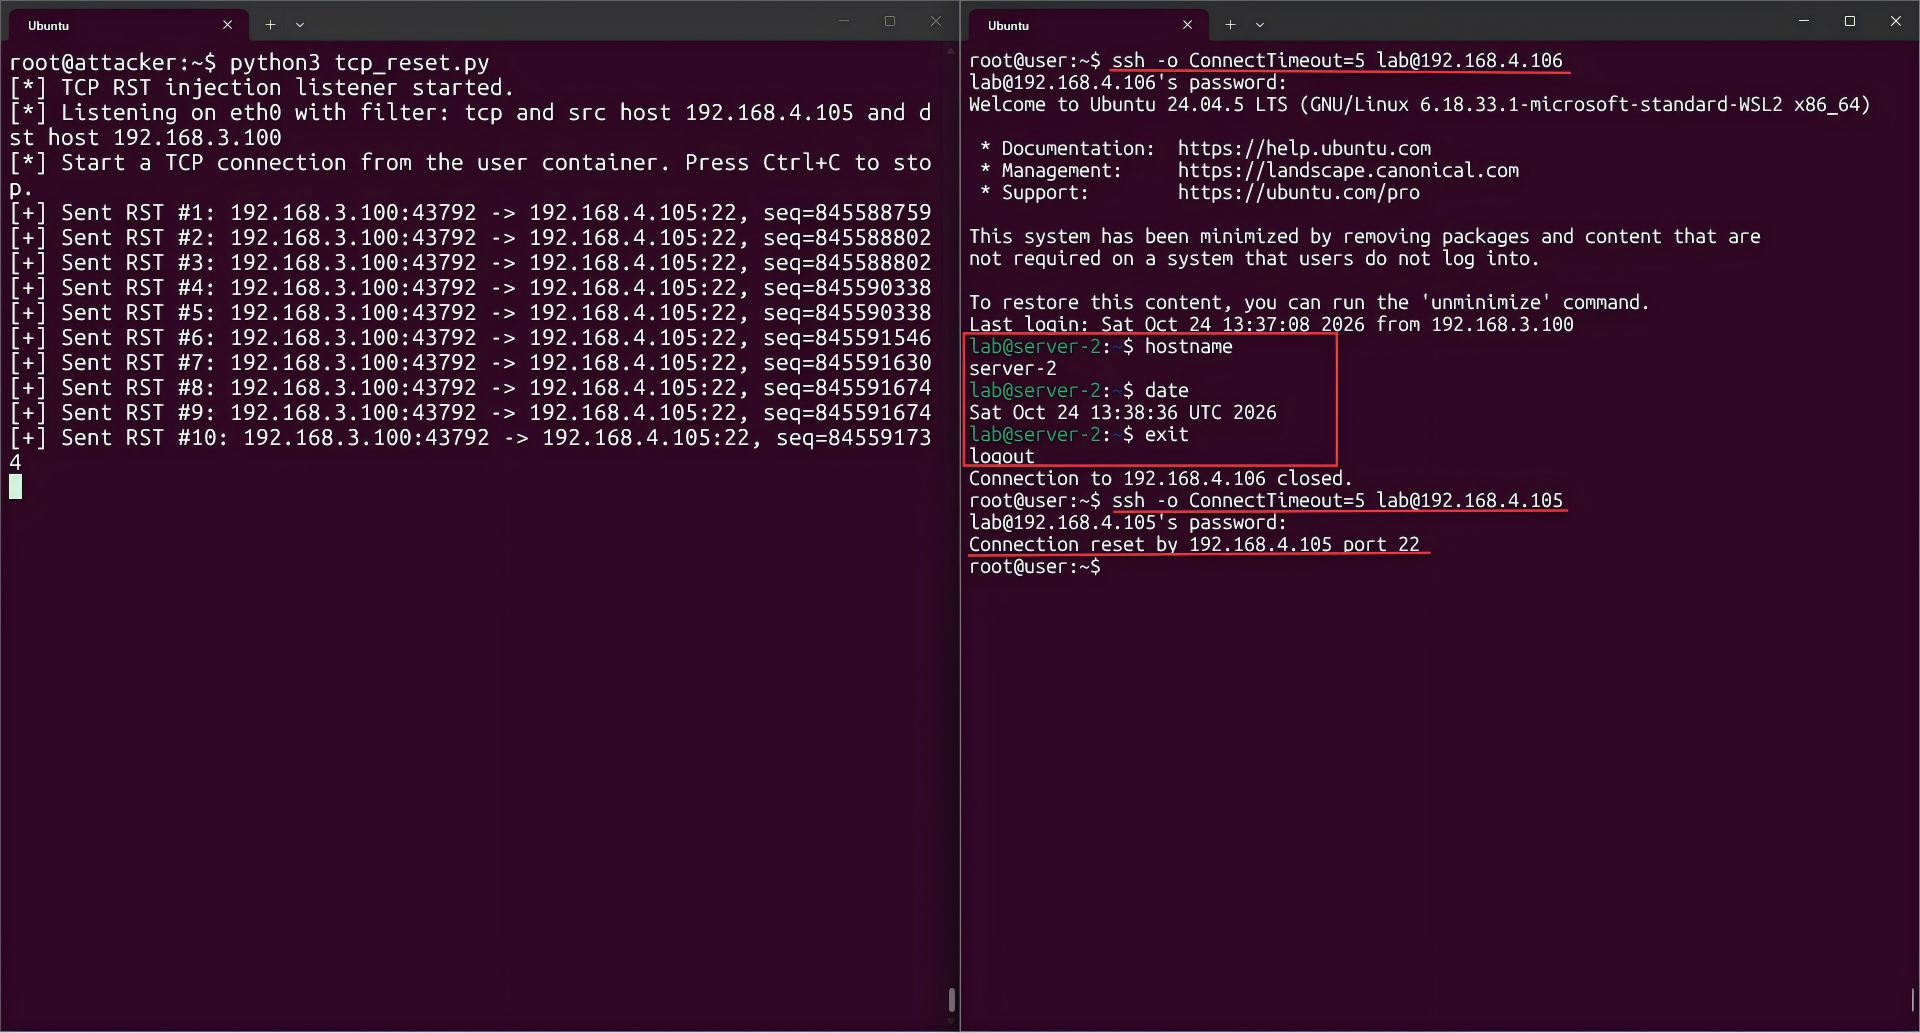
\includegraphics[trim=720bp 0 0 0,clip,width=0.88\linewidth]{figures/task3/ssh_after_attack(1).png}
    \caption{\texttt{TCP} 重置期间，正常服务器 \texttt{SSH} 可用，受害者服务器连接被重置}
    \label{fig:task3-ssh-after}
\end{figure}

\texttt{FTP} 对照中，正常服务器仍能完成登录和目录查询；受害者服务器的控制连接则返回 \texttt{421 Service not available} 并关闭。Attacker 终端同时记录到发往受害者 \texttt{FTP} 端口 21 的 RST 报文，如图~\ref{fig:task3-ftp-after} 所示。

\begin{figure}[H]
    \centering
    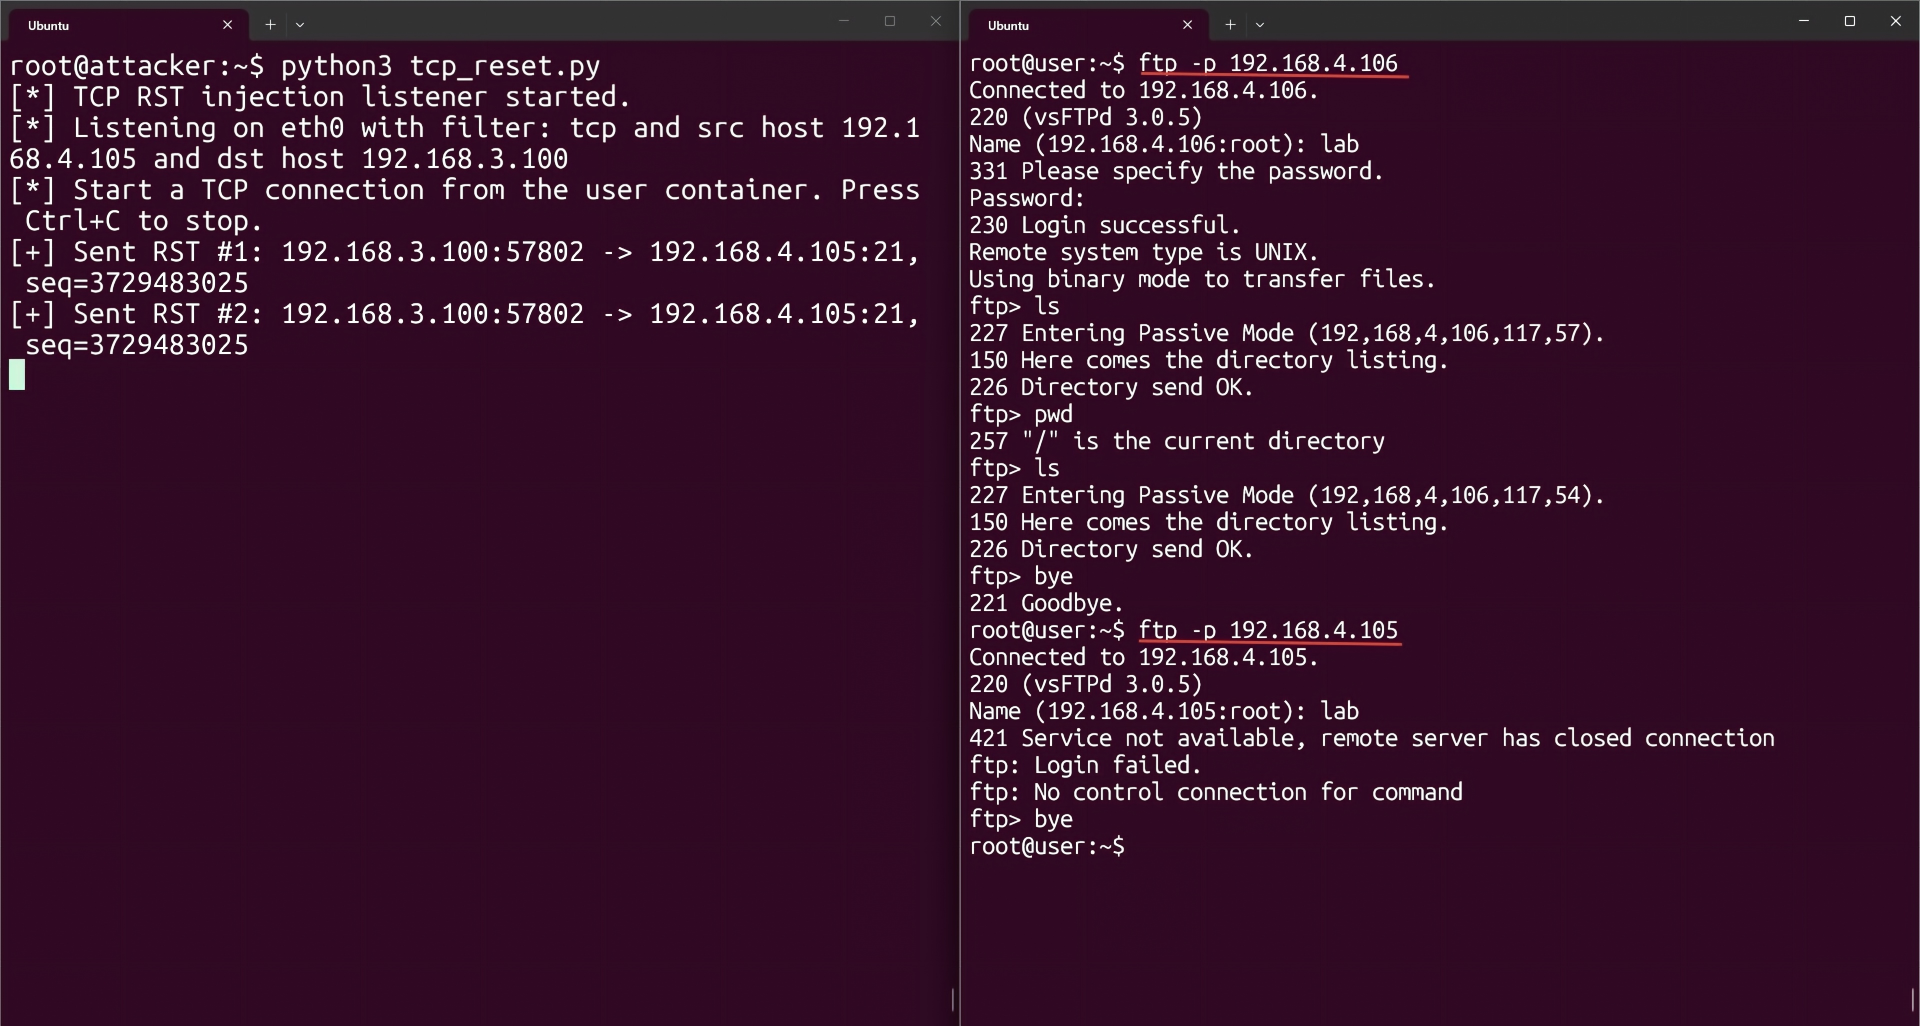
\includegraphics[width=0.98\linewidth]{figures/task3/ftp_after_attack(1).png}
    \caption{\texttt{TCP} 重置期间，正常服务器 \texttt{FTP} 可用，受害者服务器 \texttt{FTP} 连接关闭}
    \label{fig:task3-ftp-after}
\end{figure}

\subsubsection{\texttt{HTTP} 下载及响应时序}
在 \texttt{HTTP} 的攻击测试中，为了使攻击效果更显著，这里在两个 Server 上都上传了大小为 8MB 的数据文件，使用 \texttt{HTTP} 从服务器下载文件，大约需要 32s 左右的时间，足够充分体现攻击效果。
首次 \texttt{HTTP} 测试中，受害者服务器返回的页面大小为 10\,671 字节。虽然 Attacker 已经发送 RST，User 仍收到了完整页面，curl 返回状态为 0，如图~\ref{fig:task3-http-small} 所示。这表明对于传输很快结束的小响应，RST 可能在下载完成后才到达，因而未能中断该次请求。

\begin{figure}[H]
    \centering
    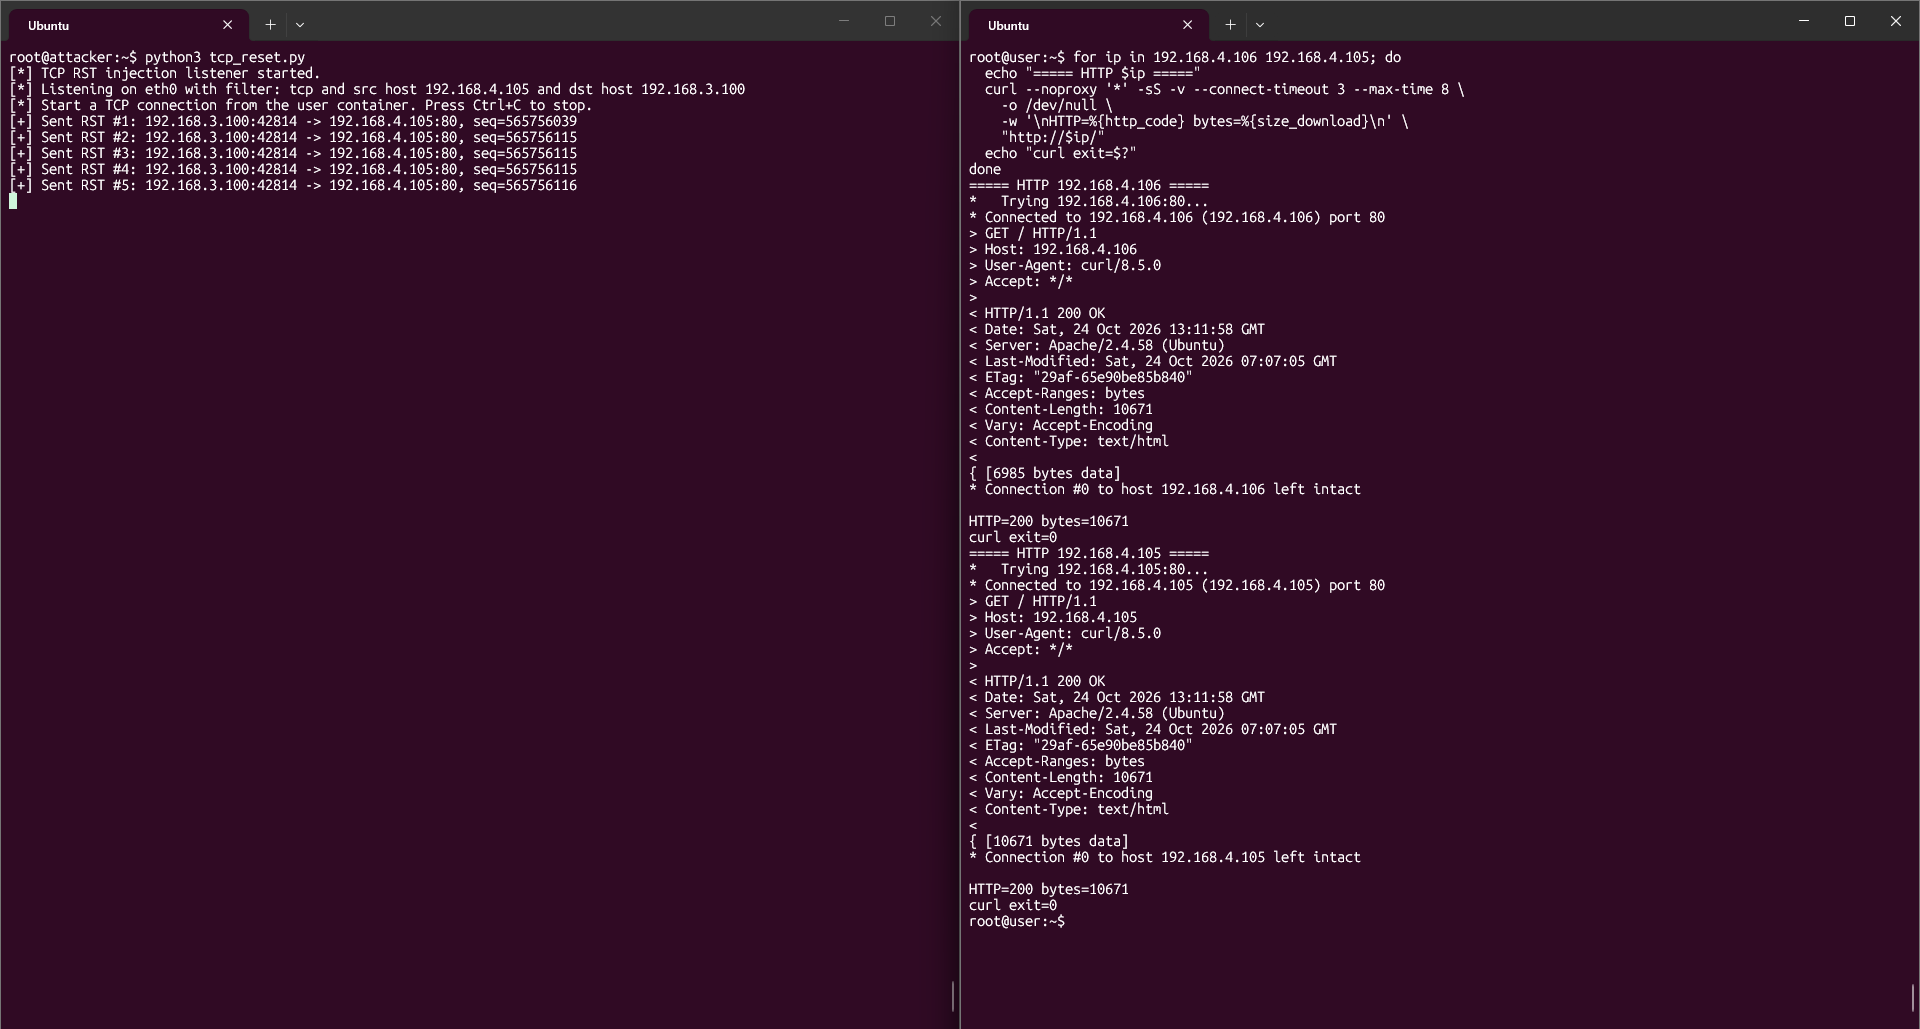
\includegraphics[width=0.98\linewidth]{figures/task3/http_short_response.png}
    \caption{小型 \texttt{HTTP} 响应在 RST 生效前完成传输}
    \label{fig:task3-http-small}
\end{figure}

为观察持续时间更长的连接，随后使用限速方式下载约 8\,MiB 的测试文件。攻击前，User 从两台服务器下载该文件均得到 \texttt{HTTP 200}，并完整收到 8\,388\,608 字节，如图~\ref{fig:task3-http-large-before} 所示。

\begin{figure}[H]
    \centering
    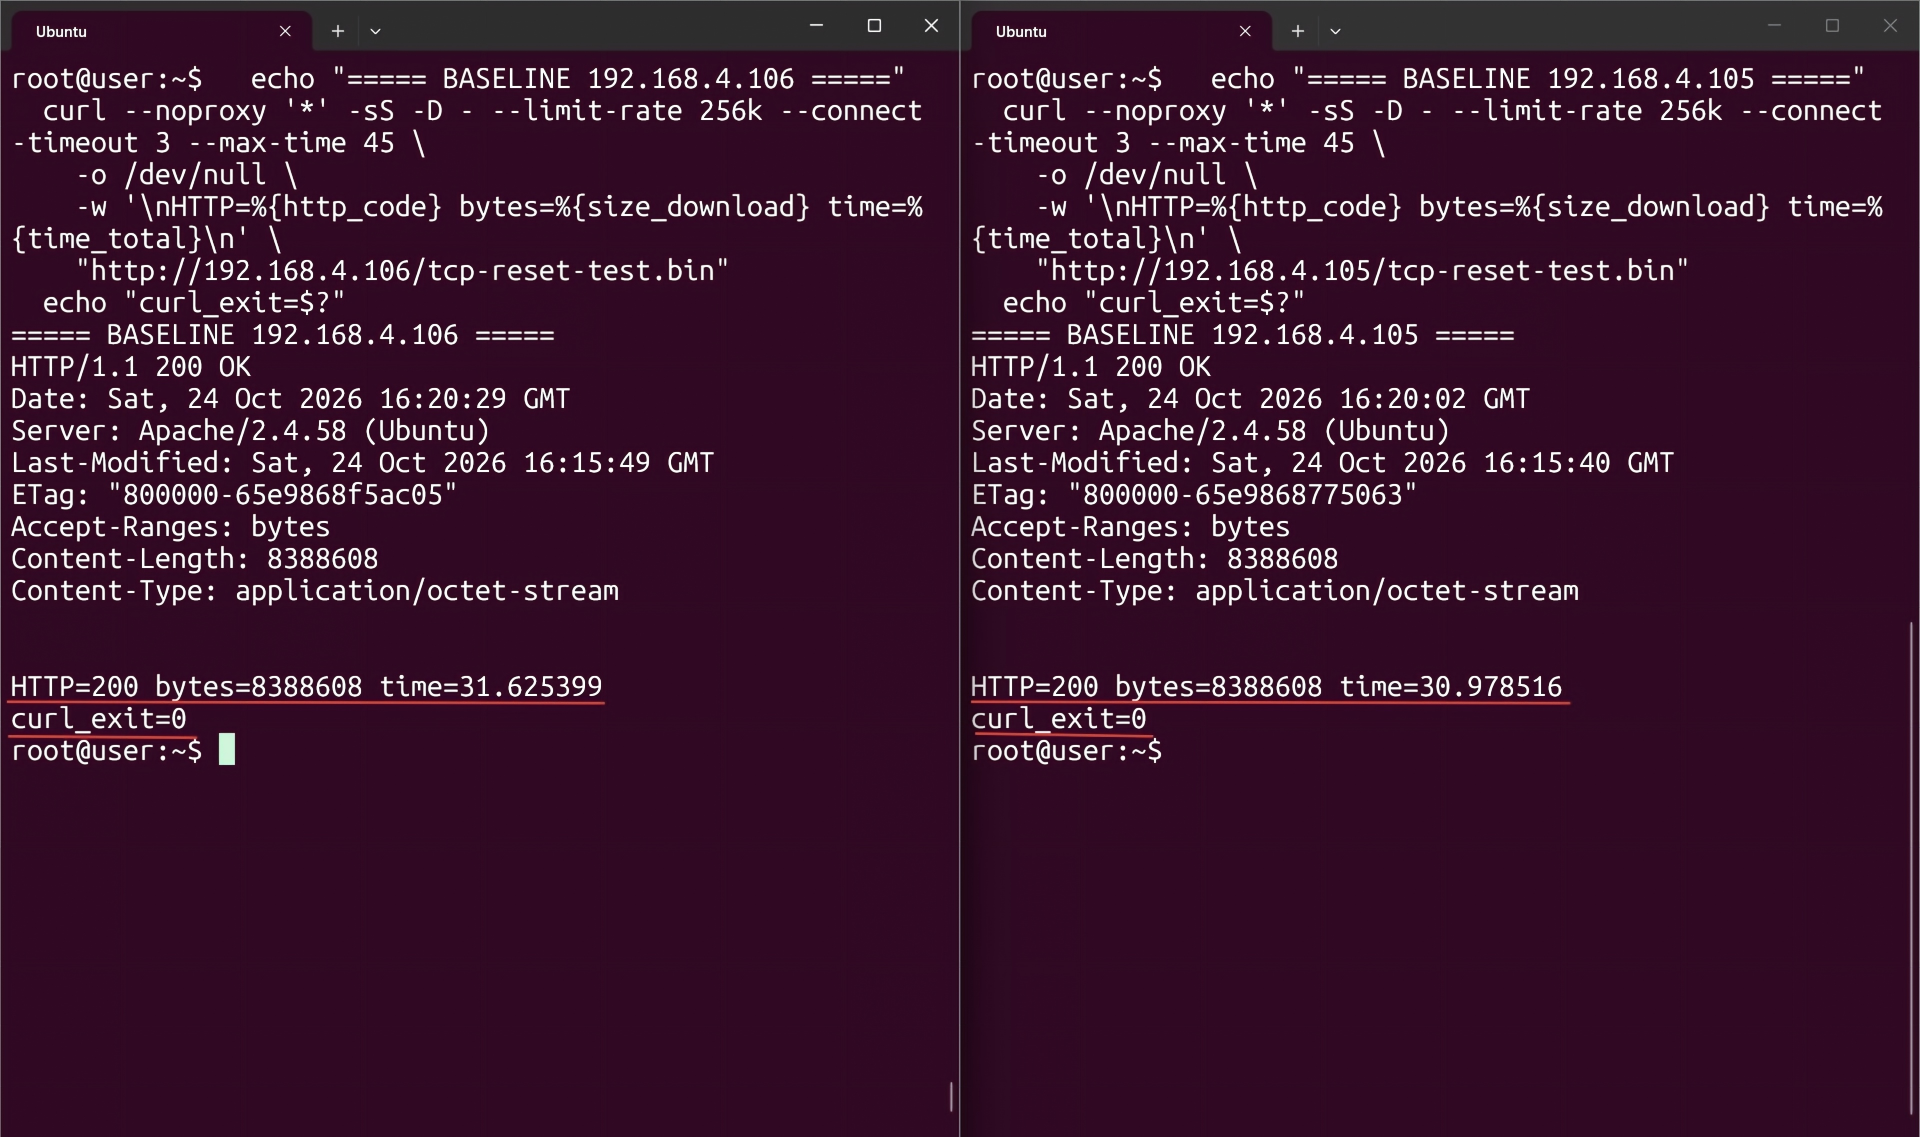
\includegraphics[width=0.98\linewidth]{figures/task3/http_large_before_attack(1).png}
    \caption{攻击前，User 均能完整下载两台服务器提供的测试文件}
    \label{fig:task3-http-large-before}
\end{figure}

启动 RST 监听后，正常服务器的下载仍完整结束，curl 返回状态为 0；从受害者服务器下载时，连接被重置，只收到 2\,725\,685 字节，curl 返回状态为 56。对照结果和 Attacker 的 RST 发送记录见图~\ref{fig:task3-http-after}。

\begin{figure}[H]
    \centering
    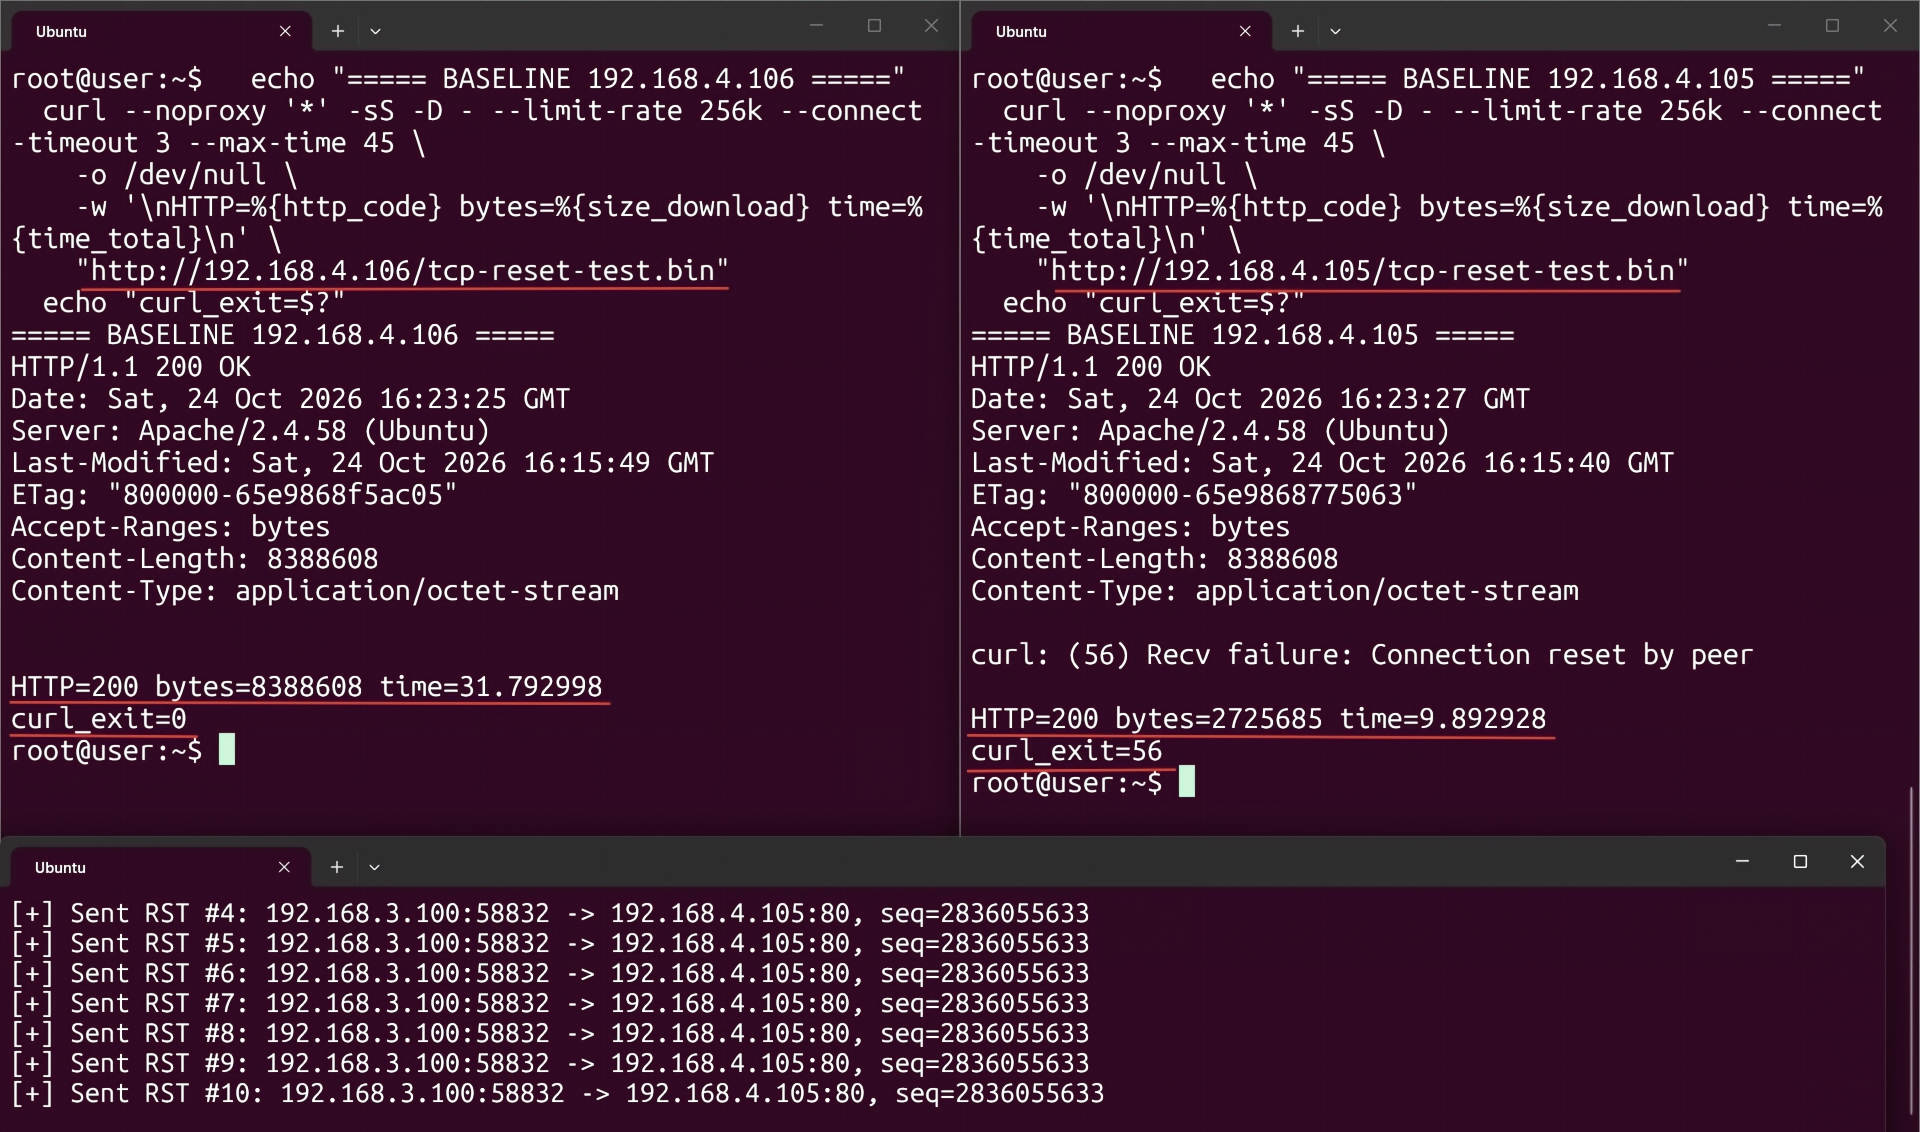
\includegraphics[width=0.98\linewidth]{figures/task3/http_reset_effect(1).png}
    \caption{限速 \texttt{HTTP} 下载时，受害者服务器连接中断，正常服务器下载完成}
    \label{fig:task3-http-after}
\end{figure}

\subsection{停止攻击后的恢复验证}

停止 Attacker 上的监听脚本后，再次从受害者服务器下载同一测试文件。User 收到完整的 8\,388\,608 字节，curl 返回状态为 0，说明停止发送伪造 RST 后，受害者服务器的 \texttt{HTTP} 连接恢复正常，如图~\ref{fig:task3-recovery} 所示。

\begin{figure}[H]
    \centering
    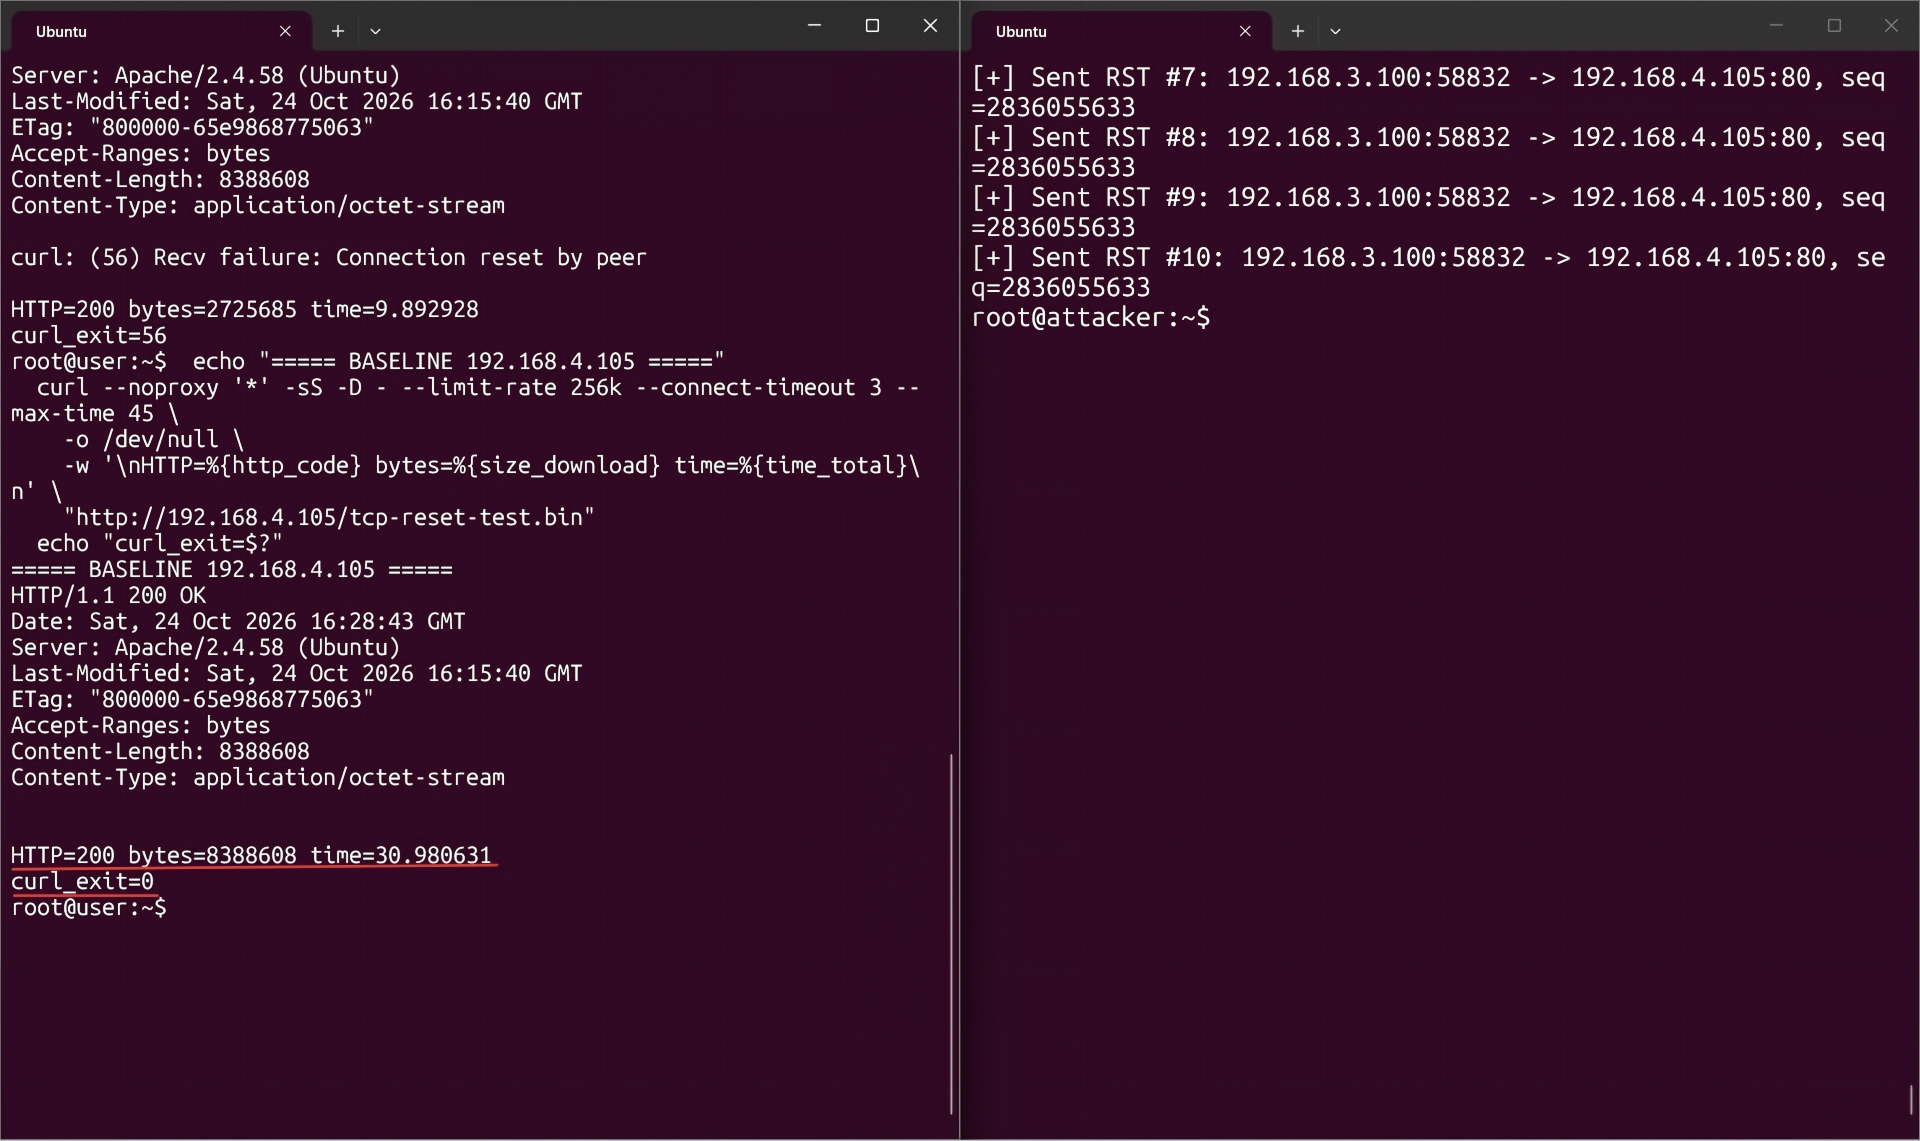
\includegraphics[trim=0 0 576bp 0,clip,width=0.76\linewidth]{figures/task3/http_recovery(1).png}
    \caption{停止 RST 监听后，受害者服务器的完整 \texttt{HTTP} 下载恢复}
    \label{fig:task3-recovery}
\end{figure}
